\UseRawInputEncoding
\documentclass[12pt]{article}
\title{ECE 102 Homework 2}
\usepackage{subcaption}
\author{Lawrence Liu}
\usepackage{graphicx}
\usepackage{amsmath}
\setlength{\parskip}{\baselineskip}%
\setlength{\parindent}{0pt}%
\usepackage{listings}
\begin{document}
\maketitle
\section*{Problem 1}
\subsection*{(a)}
After Laplace transform we have that
$$3s^2Y(S)+19sY(s)+20Y(S)=2sX(s)-X(s)$$
$$H(s)=\boxed{\frac{2s-1}{3s^2+19s+20}}$$
\subsection*{(b)}
$$X(s)=\frac{2}{2s+1}e^{-3s}$$
$$Y(s)=H(s)X(s)$$
$$Y(s)=e^{-3s}\frac{(2s-1)}{(3s^2+19s+20)(s+\frac{1}{2})}$$
$$Y(s)=e^{-3s}\frac{(2s-1)}{(3s+4)(s+5)(s+\frac{1}{2})}$$
$$Y(s)=\frac{e^{-3s}}{3}\frac{(2s-1)}{(s+\frac{4}{3})(s+5)(s+\frac{1}{2})}$$
$$Y(s)=\frac{e^{-3s}}{3}\left(\frac{-\frac{5}{3}}{s+\frac{4}{3}}+\frac{-11}{s+5}+\frac{-2}{s+\frac{1}{2}}\right)$$
$$Y(t)=\boxed{-\frac{5}{9}e^{-\frac{4}{3}(t-3)}u(t-3)-\frac{11}{3}e^{-5(t-3)}u(t-3)-\frac{2}{3}e^{-\frac{t-3}{2}}u(t-3)}$$
\section*{Problem 2}
\subsection*{(a)}
The system response function is
$$h(s)=\frac{2s^2-14s-16}{s^2+6s^2+11s+6}$$
$$h(s)=\frac{2}{s+2}\frac{1}{s+3}(s-8)$$
Thus the system looks like
\begin{center}
\begin{figure}[h]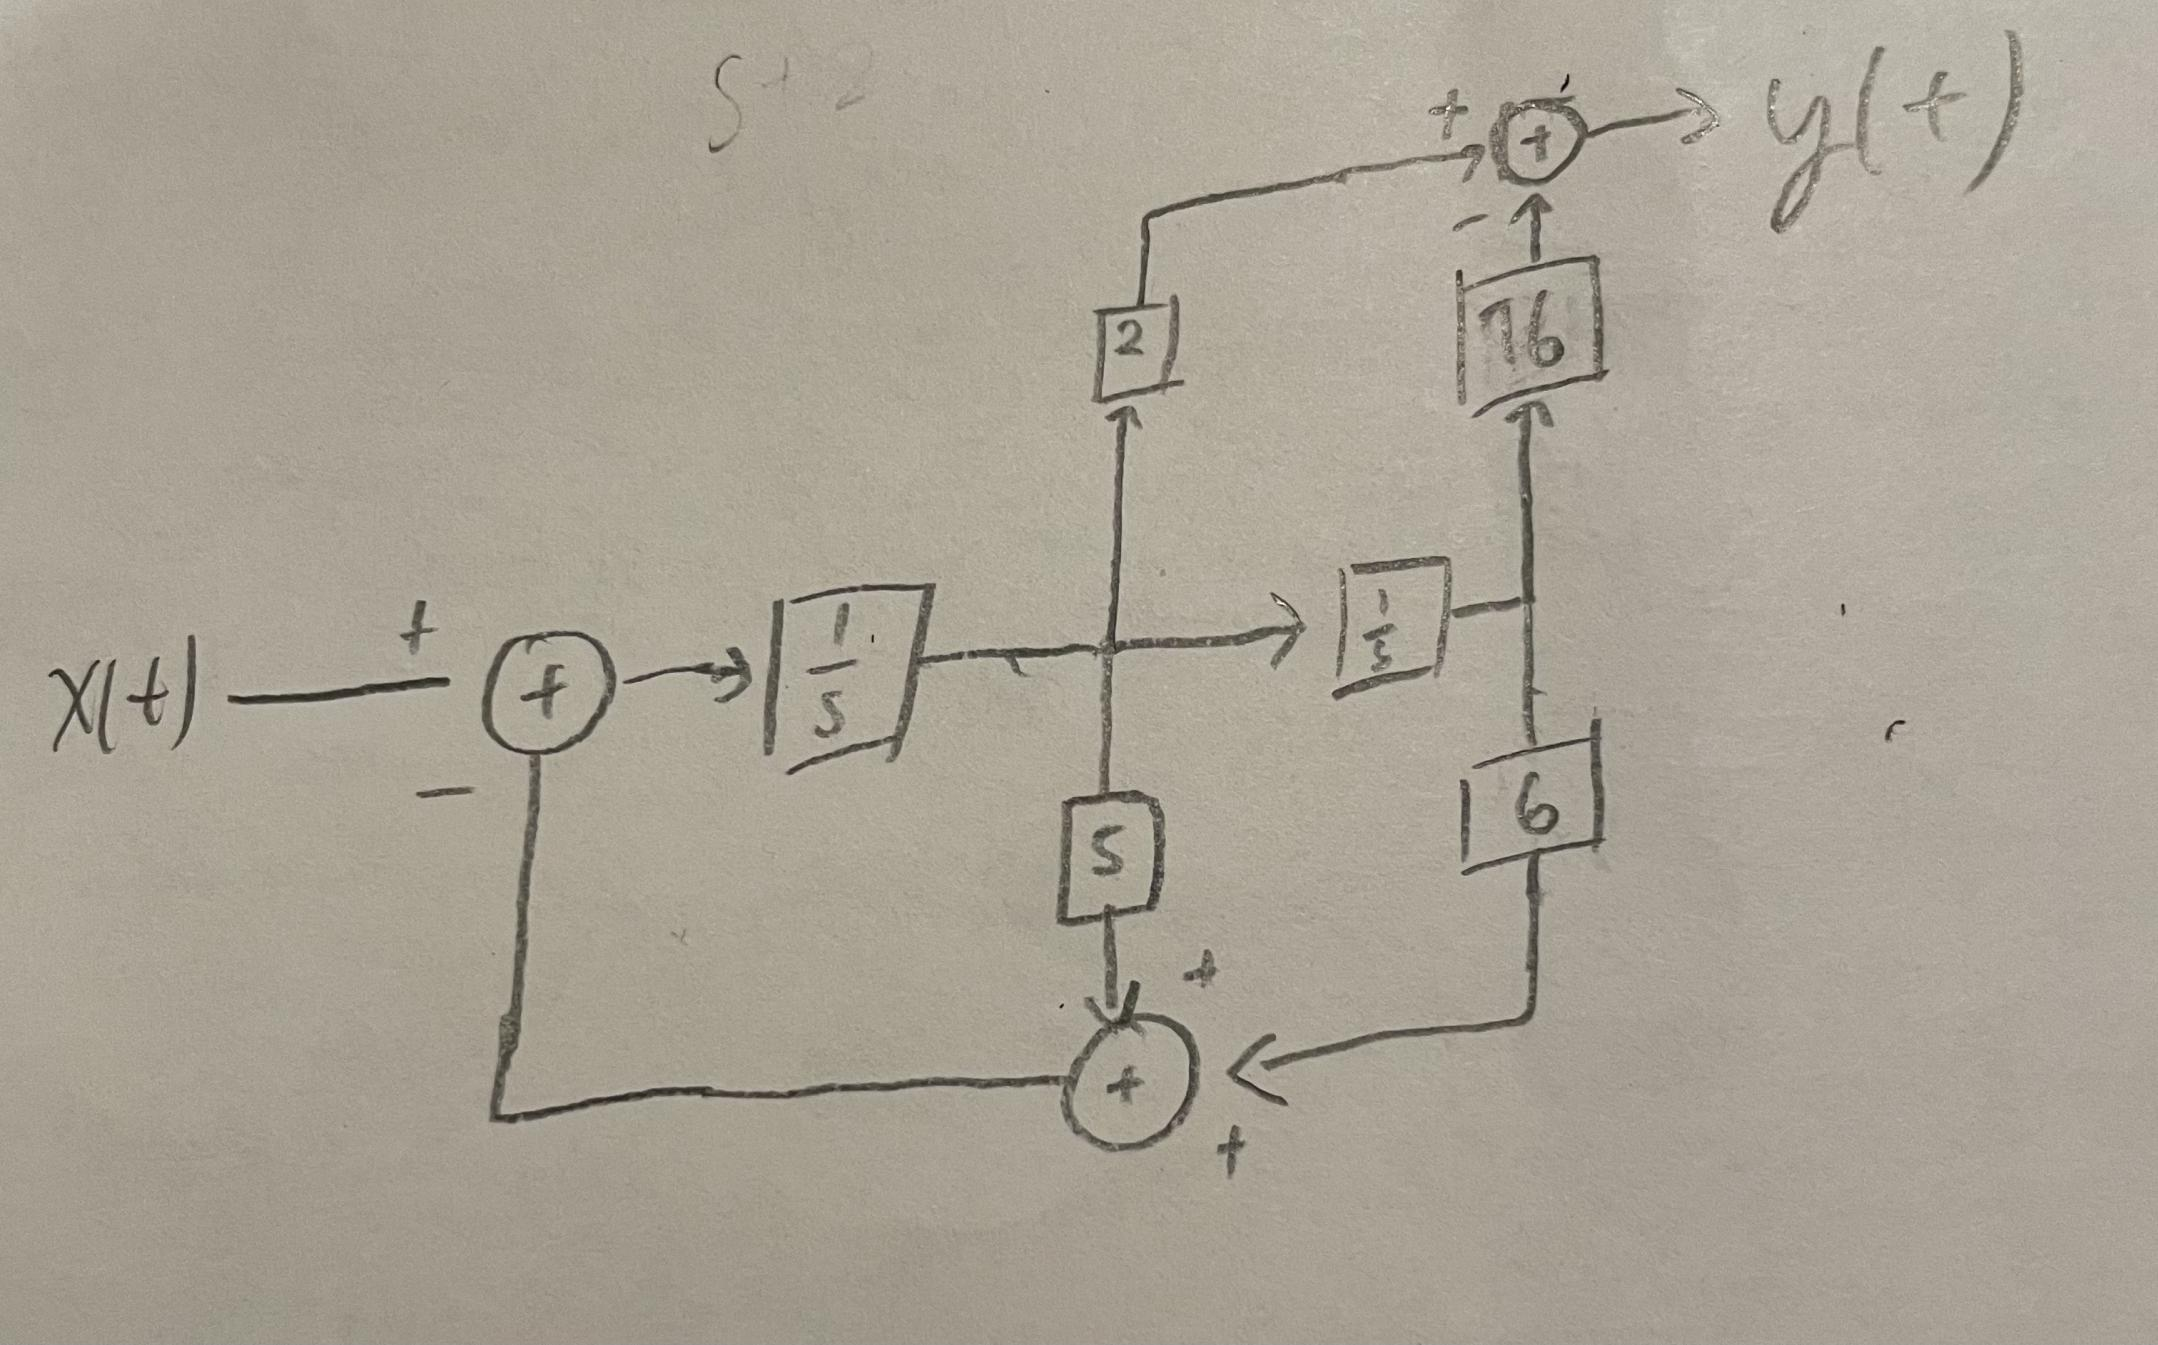
\includegraphics[width=10cm]{fig1}
\end{figure}
\end{center}
\subsection*{(b)}
\begin{center}
\begin{figure}[h]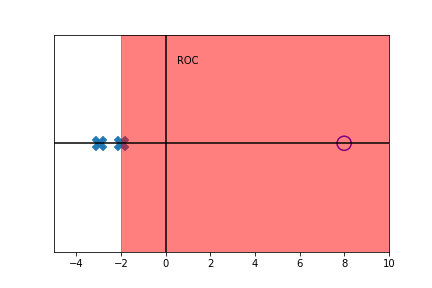
\includegraphics[width=10cm]{fig2}
\end{figure}
\end{center}
This converges since the roc includes $s=0$
\subsection*{(c)}
$$X(s)=\frac{1}{s}\left(e^{2s}-e^{-2s}\right)$$
\begin{align*}
Y(s)&=X(s)H(s)\\
&=\left(e^{2s}-e^{-2s}\right)\frac{2(s-8)}{s(s+2)(s+3)}\\
&=-\left(e^{2s}-e^{-2s}\right)\left(\frac{16}{s}+\frac{20}{s+2}+\frac{22}{s+3}\right)
\end{align*}
Reverse Laplace transforming we get that

$$y(t)=\boxed{\left(16+20e^{-2(t-2)}+22e^{-3(t-2)}\right)u(t-2)-\left(16+20e^{-2(t+2)}+22e^{-3(t+2)}\right)u(t+2)}$$
\section*{Problem 3}
\subsection*{(a)}
Let $a(t)$, $b(t)$, and $c(t)$ be determined as depicted in the drawing below
\begin{center}
\begin{figure}[h]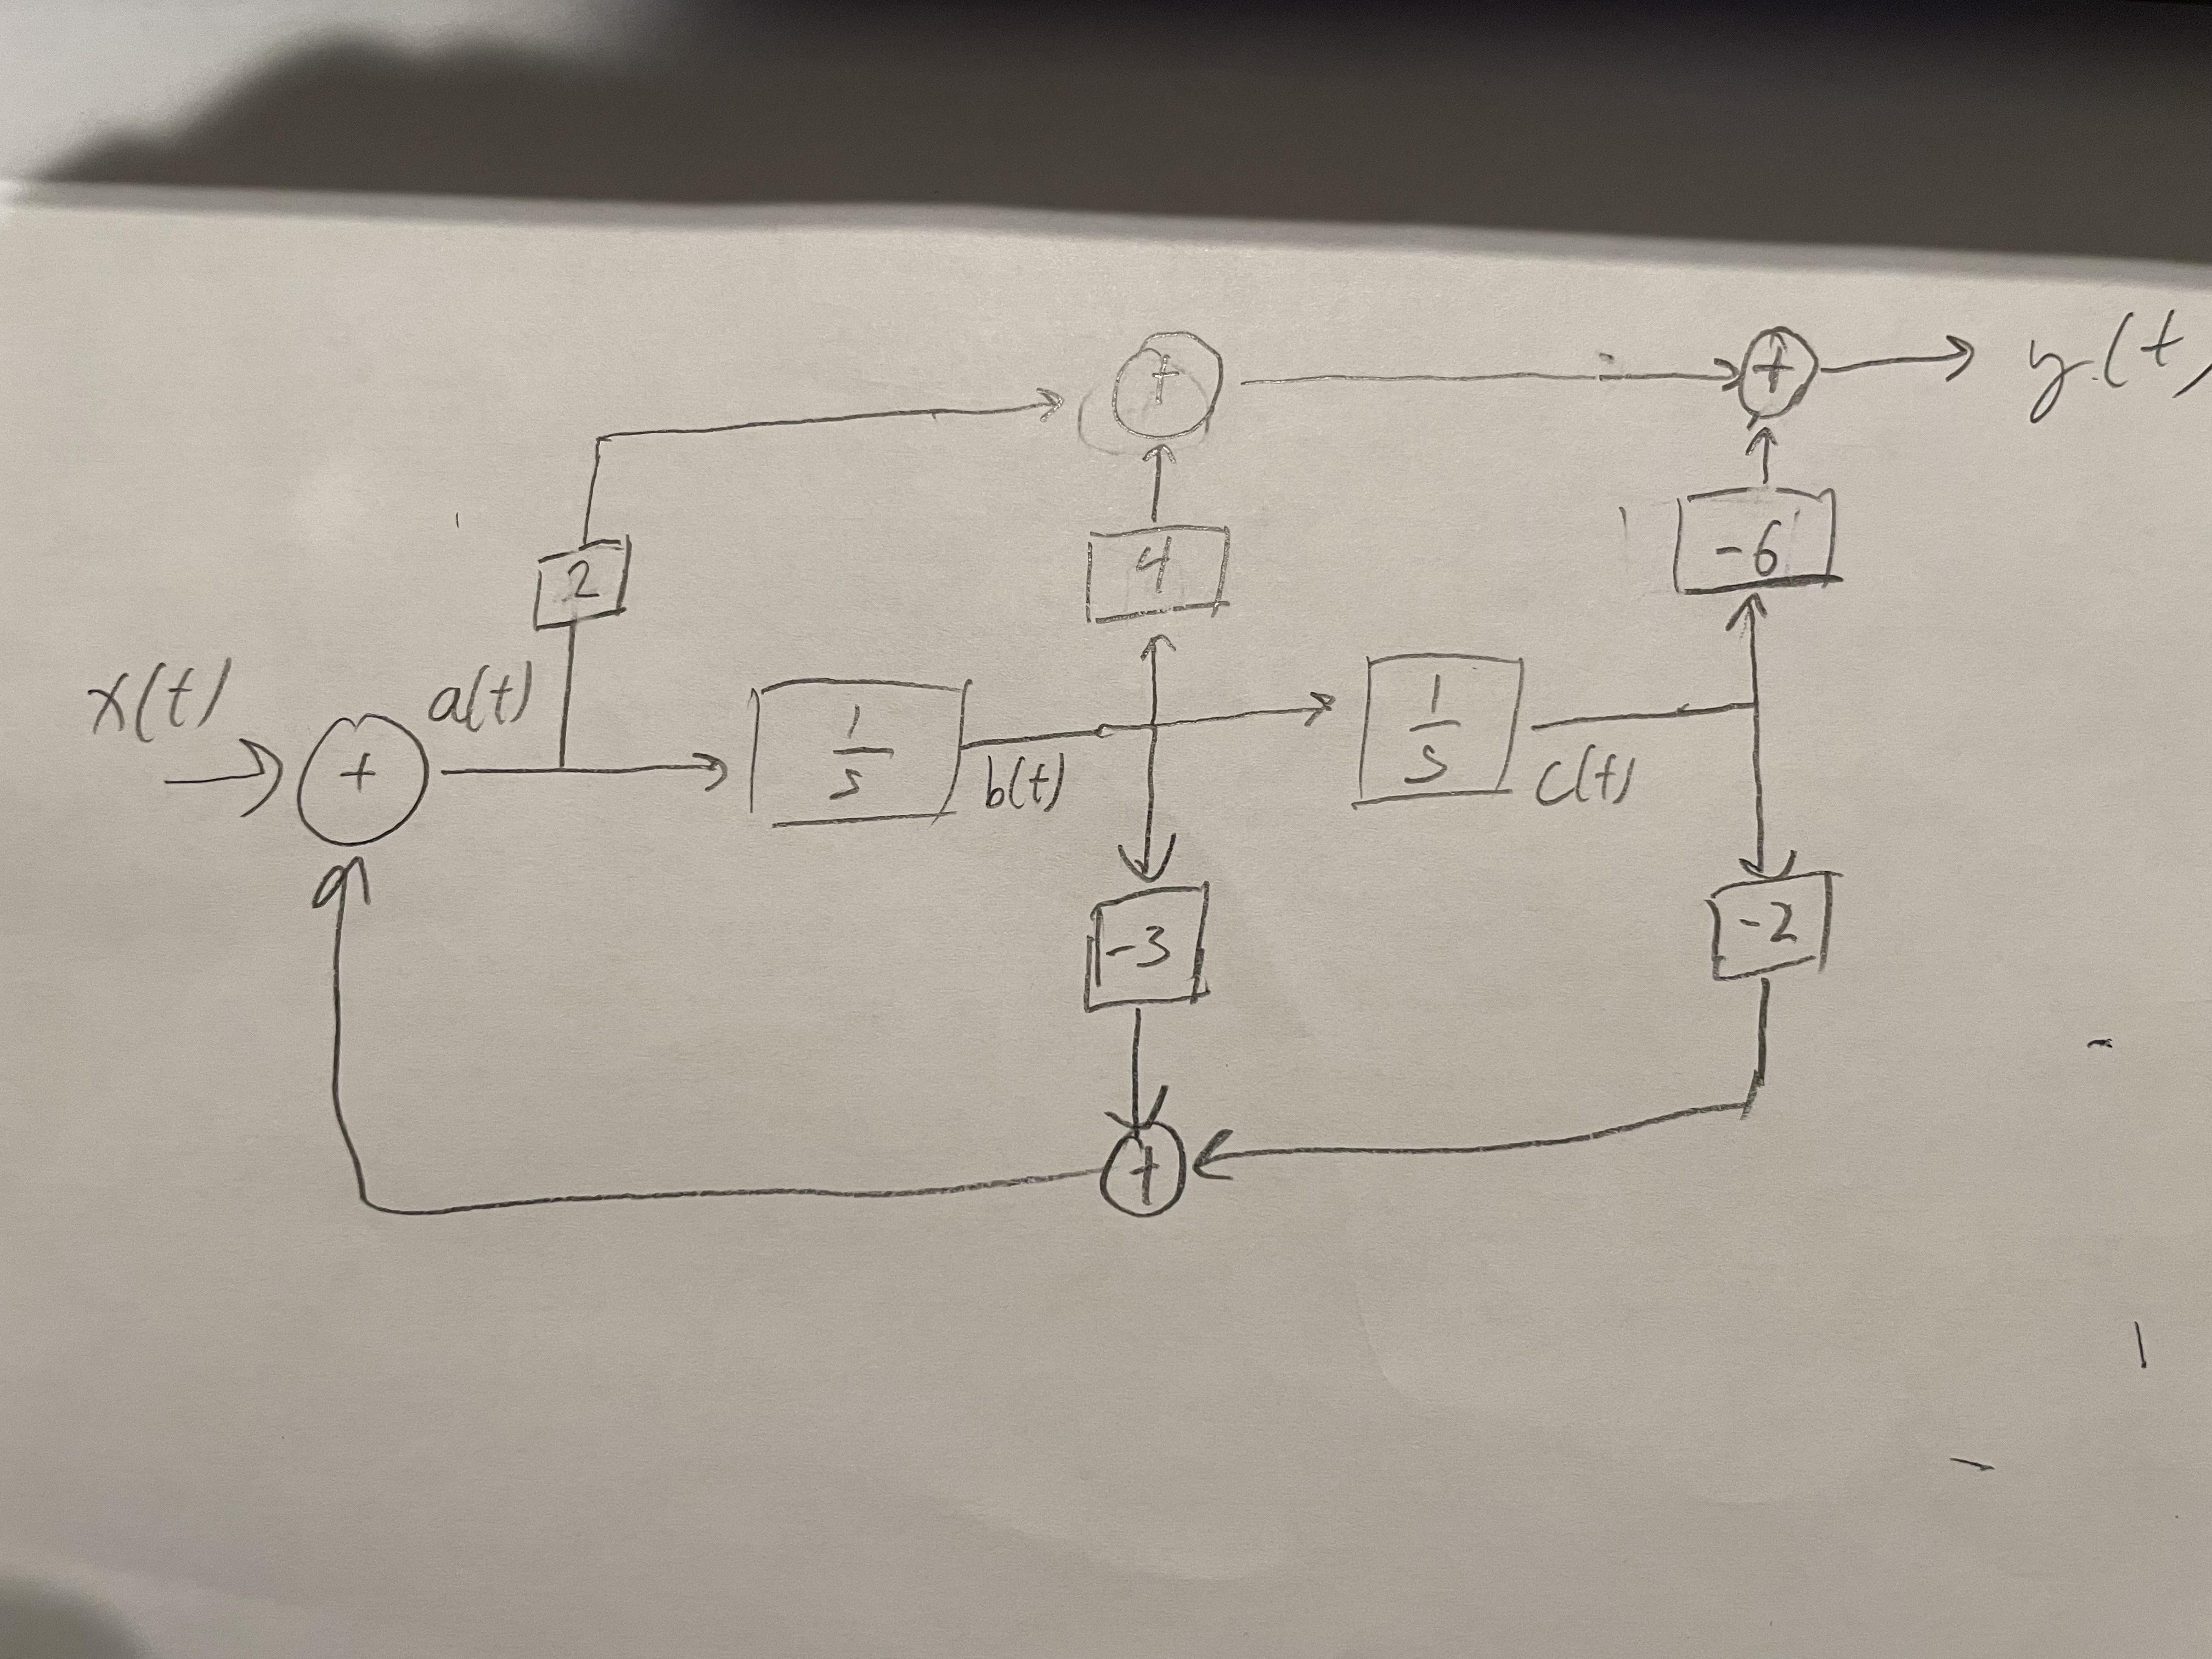
\includegraphics[width=10cm]{fig3}
\end{figure}
\end{center}

Therefore in the $s$ domain we have
$$A(s)=X(s)-3B(s)-2C(s)$$
$$B(s)=\frac{1}{s}A(s)$$
$$C(s)=\frac{1}{s}B(s)=\frac{1}{s^2}A(s)$$


Therefore we have that 
$$A(s)=X(s)-\frac{3}{s}A(s)-\frac{2}{s^2}A(s)$$
$$A(s)=X(s)\frac{1}{1+\frac{3}{s}+\frac{2}{s^2}}$$
$$A(s)=X(s)\frac{s^2}{s^2+3s+2}$$
Thus we have that 
\begin{align*}
Y(s)&=2A(s)+4B(s)-6C(s)\\
&=X(s)\frac{s^2}{s^2+3s+2}\left(2+4\frac{1}{s}-6\frac{1}{s^2}\right)\\
&=X(s)\frac{s^2}{s^2+3s+2}\frac{2s^2+4s-6}{s^2}\\
&=X(s)\frac{2s^2+4s-6}{s^2+3s+2}
\end{align*}

Thus we have that
$$H(s)=\boxed{\frac{2s^2+4s-6}{s^2+3s+2}}$$
\subsection*{(b)}
We have that
$$H(s)=\frac{Y(s)}{X(s)}=\frac{2s^2+4s-6}{s^2+3s+2}$$
$$Y(s)(s^2+3s+2)=X(s)(2s^2+4s-6)$$
Inverse laplace transforming we get that
$$\boxed{\frac{d^2y(t)}{dt^2}+3\frac{dy(t)}{dt}+2y(t)=2\frac{d^2x(t)}{dt^2}+4\frac{dx(t)}{dt}-6x(t)}$$
\subsection*{(c)}
\begin{align*}
H(s)&=\frac{2s^2+4s-6}{s^2+3s+2}\\
&=

\end{align*}
\end{document}